\documentclass{mcmthesis}
\bibliographystyle{plain}
\mcmsetup{CTeX = false,   % 使用 CTeX 套装时,设置为 true
        tcn = H155, problem = B,
        sheet = true, titleinsheet = true, keywordsinsheet = true,
        titlepage = false, abstract = true}
\usepackage{palatino}
\usepackage{lipsum}
\usepackage[UTF8, nocap]{ctex}
\usepackage{array}
\usepackage{float}
\usepackage{graphicx}
\usepackage{subfigure}
\usepackage{booktabs}
%\usepackage{ctex}
%\usepackage{CJK}
\title{An Insight of a Puzzle Game}
\author{}
\date{\today}

\begin{document}

	\begin{abstract}
		
		The game enriched our childhood, and puzzle games like Wonderland not just beautified children's lives but cultivated their logical thinking ability. The core issue in designing such a game is how to determine the difficulty and mode of solving it.
		
		When we carefully analyze the game, we find that the critical point is how to capture the impact of each constraint in it effectively. Therefore, we divide the constraints into two categories(\textbf{Target-based constraint} and \textbf{Relation-based constraint}) and propose to use two indicators(\textbf{Free Degree of Choices} and \textbf{ Free Degree of Species}) to represent the effect of these two constraint types in the game respectively.
		
		Based on the above two indicators, we have proposed an objective Difficulty Evaluation Model, which can avoid human subjectivity. And an algorithm is applied to solve the problem more efficiently by using the Free Degree of Choices which can correctly represent the indirect information.
		
		Many factors affect the difficulty of a game, but several factors are prime indicators of dealing with such puzzle games. Take the wonderful island as an example: the type of animal, the number of grids, and the number of constraints. \textbf{To transform the actual meaning of the constraint into statistical significance}, we use the two free degrees above, which constitutes the \textbf{Contribution Index}, to capture the impact of the actual meaning of the constraints. The primary indicators and the contribution index form our difficulty evaluation model. Through sensitivity analysis, our model can well apply to the evaluate the difficulty of such games.
		
		For the solution of the problem, because the change of the free degree can adequately represent the use of the constraint, we propose a \textbf{Improved Search Model based on Free Degree}. The main purpose is to orderly traverse the species so as to better use constraints to reduce the number of combinations that the algorithm needs to traverse.
		
		Based on our Difficulty Evaluation Model and ISMDF, we designed our new game - "YES SIR!" The game is based on city planning, with the real urban layout as the chessboard of the game, allowing players to locate infrastructures in various blocks in the city. Our game is more realistic and has more possibilities and scalability.
		
		
		
		
		
		\begin{keywords}
			Free Degree; Difficulty Evaluation Model; Improved Search Model based on Free Degree(ISMFD); Information Utilization;
		\end{keywords}
	\end{abstract}

	\maketitle
	\setcounter{tocdepth}{2}
	\tableofcontents
	
	\newpage
	\section{Introduction}
		
		The game enriches our lives. Games not just delight us, it also cultivates our courage to go forward, completing missions and also allows us to experience the great joy of breaking through the difficulties.
		
		Defining the difficulty of games has always been an important research topic in the game industry, because it is a prerequisite for a game to succeed.
		
		
		
		\subsection{Background}
		
			Wonderful Island is a game for children above six years old aiming at training logical thinking ability and cultivating intelligence. It has a cute background story for children to immerse in. Regardless of how the background is set, the core is to examine the sense of permutation and combination, the purpose is to solve complex problems in given operating spaces and under some constraints.
			
			This paper is based on the ‘Wonder Island’ game, and
			studies in abstracting the model from it, and defining game’s difficulty, developing an algorithm to cope with this type of game, and finally proposing a novel new game.
		
			
		\subsection{Overview of Our Work}
		
			First, we find a few key points in this question:
					
			\begin{itemize}
				\item How to define the difficulty of the game and how to convert the difficulty into level.
				
				\item How to use algorithm or model to find the number of feasible solutions of the problem more quickly.
				
				\item How to use analsis above to propose a new and novel game.
			\end{itemize}
			
			\textbf{On the basic of above discussion, we may boil down the tasks to the follow four steps:} 
			
			\begin{itemize}
				\item First, we define the difficulty.
				
				\item[-] We carefully analyzed the literature and found that there are \textbf{three main indicators} that will greatly affect the difficulty of the game, named \textbf{Basic Indicator}. We consider these three indicators into our difficulty evaluation model.
				
				\item[-] Based on the unique characteristics of the game of "Wonderful Island", we define the \textbf{Contribution Index} to capture the difficulty changes caused by the unique constraints of this game, and combine the two parts as our Difficulty Definition Model.
				
				
				\item Secondly, we optimize the search algorithm based on Free Degree of Choices to better use the information of constraints as much as possible. Based on this, we propose an algorithm: Improved Search Model based on Free Degree.
				
				\item Then, based on the model and analysis above, we proposed a novel game "Yes, Sir". It isn't similar to "Wonder Island" in form, but they are alike in spirit. And our game has a more realistic background and a higher freedom of operation.
			
				\item Finally, we have provided a memo for readers to promote our game.
			\end{itemize}
		
			
			
	
	\section{Fundamental Assumptions}
		\begin{itemize}
			\item There is no more than one animal species without any restrictions.
			
			\item Limiting the type of fruit in each cell in the game is fixed.
			
			\item When two species must be neighbors, this restriction requires that each one of those two species must be neighbor to the other speices one.
			
			\item Each constraint is non-repetitive and effective.
			
			\item Neighbor relation means that there must be one side as the common side.
			
		\end{itemize}

	\section{Difficulty Evaluation Model}
	
		In this part, we focus our attention on how to determine difficulty evaluation system. In the troditional field, basic index such as magnitude of the combined problem are used to evalue difficulty, which is a way of taking time complexity into considering.
		
		According to the Game: Wonder Island, we use the available information to construct a new dificulty evaluation model approprate for this game.
		
		\begin{equation}
		D = GN \times AN \times RN \times Contribution\ Index
		\end{equation}
		
		\subsection{Basic indicator}
	
			For a given problem of logic analysis, there are many factors that affect the difficulty of solving it. There may be a connection between various factors. According to our observation, we have identified three independent basic influencing factors: the number of grids, restrictions and possible choices (animals possibly to be selected in games). But why these three factors?
		
			\subsubsection{GN: Number of Grids}
	
				For a given logical analysis problem, the more units involved in the problem, the higher the difficulty. Obviously, because a larger number of computing units means higher time complexity, that is, the number of cells is proportional to the difficulty of the problem.
				
			
			\subsubsection{AN: Number of Animals}
				
				Similar to the above analysis, the more difficult questions often mean more types of animals are involved in. Because the more animal species means more choices, more possibilities, more hidden impossibilities need to be considered, and more time is needed to solve the problem. The number of animal species also has a positive impact on the difficulty.
				
				
			\subsubsection{RN: Number of Constraints}
			
				The constraints are statistically significant, when we do not consider the internal differences of the constraints. The more restrictions need  more time to thinking about how to meet constraints once for all. Therefore, the number of restrictions has a positive relationship with the difficulty.	
				

				
		\subsection{Contribution Index}
			
			For typical game based on permutation and combination problem, the difficulty evaluation model based on basic indicator is enough. But for this Wonder Island issue, we add an correction index, "Contributon Index", to make the definition more robust.
			
			Because the constrains not just have statistical significance, they also have practical significance, that means every single constrain has a unique affect to games difficulty.
			
			This difference is not only reflected in the size of the constraints on the difficulty contribution, but also in the direction of the contribution to the difficulty(some constrains make problem more difficult and other make it easier). Therefore, we use the contribution index to measure the average contribution rate of the constraint to the difficulty.
			
			
			By Summarizing, we could divid constraints into two types, one is the constraint between grids and animals, and the other is the constraint between different kinds of animals. 
			
			In order to better describe these two constraints, we use the free degree of choices($\mathrm{F_{choices}}$) and the free degree of species($\mathrm{F_{species}}$) to capture the contribution of the two constraints to the difficulty. The contribution index is obtained by the ratio of free degree of choices to free degree of species.
			
			\begin{equation}
			Contribution\ Index = \frac{F_{choices}}{F_{species}}
			\end{equation}
		
			\subsubsection{Free Degree of Choices}
			
				\begin{figure}[h]
					\small
					\centering
					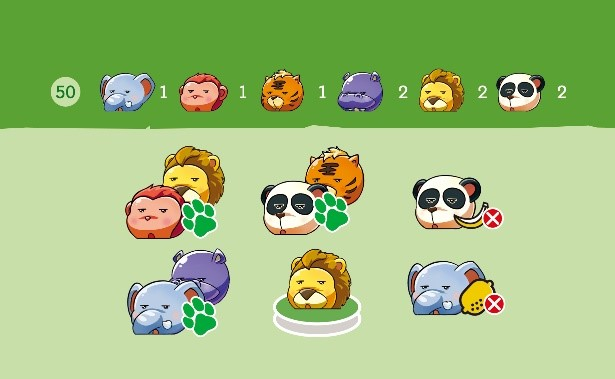
\includegraphics[width=12cm]{level50.jpg}
					\caption{Level-50} \label{fig:level50}
				\end{figure}
			
				Let's focus on the constraint in the lower right corner.
				
				\begin{center} 
					\emph{"The elephant cannot eat lemons."}
				\end{center}
			
				This constraint can help us determine the location of the animal and help to reduce the difficulty of the problem by increasing the correlation between the animal and the grid. The contribution of this constraint to difficulty is captured by the free degree of choices($\mathrm{F_{choices}}$):
				
				\begin{equation}
				F_{choices} = \sum_{i=1}^n S(i)
				\end{equation}
				
				Where $S(i)$ is number of possible localtions for animal i and $n$ is the number of animal species in a game.
				
				\begin{equation}
				S(i) = \sum_{k=1}^m N(i,k)
				\end{equation}
				
				$$ N(i,k)=\left\{
				\begin{aligned}
				1 & , & grid\ is\ possible\ choice\ for\ animal \\
				0 & , & grid\ is\ not\ possible\ choice\ for\ animal
				\end{aligned}
				\right.
				$$
				
				Where $N(i,k)$ represent the state between animal i and chosen grid (are grid k is a possible localtion for animal i?)
				
				We use the senario level-50 to display the calculation process:
				
				We first number nine grids, and according to the problem, we could related each grid to three features which is the bridge between animals and grids.
				
				\begin{figure}[h]
					\small
					\centering
					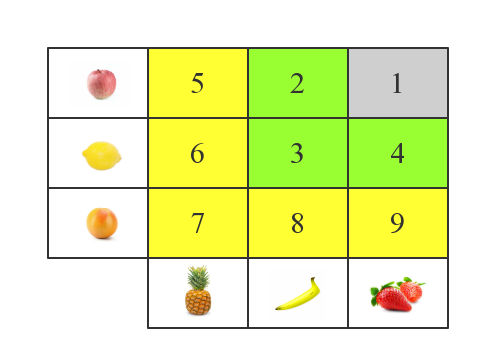
\includegraphics[width=12cm]{grids.png}
					\caption{Grids} \label{fig:grids}
				\end{figure}
			
				For instance, grid(9) has three features: Strawberry, Orange and Level-3.
				
				\begin{itemize}
					\item \emph{"Lions must be the neighbors of the monkey."}
					\item \emph{"Hippos must be the neighbors of the elephants."}
					\item \emph{"Pandas must be the neighbors of the tigers."}
					\item \emph{"The Lions go on the second level."}
					\item \emph{"The pandas cannot eat bananas."}
					\item \emph{"The elephants cannot eat lemons."}
				\end{itemize}
			
				According to those constraints above, we could calculate the $F_{choices}$:


				\begin{equation}
					S(i)=\left\{
					\begin{aligned}
					& S (Elephant) & = & \sum _ { i = 1 } ^ { 9 } N (Elephant, i ) & = & 4 \\
					& S (Monkey) & = & \sum _ { i = 1 } ^ { 9 } N (Monkey, i ) & = & 2 \\
					& S (Tiger) & = & \sum _ { i = 1 } ^ { 9 } N (Tiger, i ) & = & 3 \\
					& S (Hippo) & = & \sum _ { i = 1 } ^ { 9 } N (Hippo, i ) & = & 14 \\
					& S (Lion) & = & 2 \cdot \sum _ { i = 1 } ^ { 9 } N (Lion, i ) & = & 4 \\
					& S (Panda) & = & 2 \cdot \sum _ { i = 1 } ^ { 9 } N (Panda, i ) & = & 12
					\end{aligned}
					\right.
				\end{equation}
				We can use a matrix to describe the whole process:
				
				\begin{figure}[h]
					\small
					\centering
					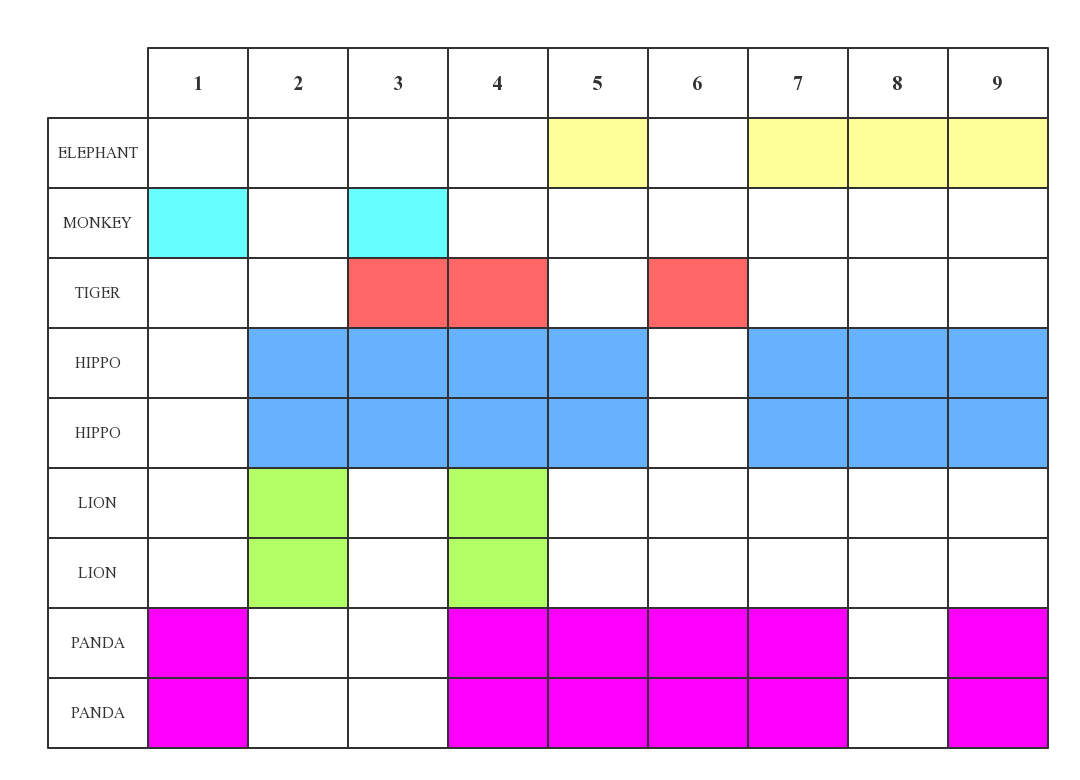
\includegraphics[width=12cm]{fchoices-level-50.png}
					\caption{Free Degree of Choices in Senario Level-50} \label{fig:fchoices-level-50}
				\end{figure}
				
				
				According to those constraints above, we could calculate the $F_{choices}$:
				
				\begin{equation}
				F_{choices} = \sum _ { i \in n } S ( i ) = 39
				\end{equation}
				
				
			
			\subsubsection{Free Degree of Species}
			
				
				\begin{center} 
					\emph{"Lions must be the neighbors of the monkey."}
				\end{center}
				
				Unlike the previous instance, this constraint can not help us to sovle the problem, con the contrary, it adds difficulty to our problem solving. Because we have to consider more to meet this constains. In fact, this kind of constrains increase all difficulty of the game by related one spices to another. The contribution of this type of constraint to difficulty is captured by the free degree of spices($\mathrm{F_{spices}}$):
				
				\begin{equation}
				F_{spices} = \sum _ { i \in n } \sum _ { j \in m } N (i) \cdot F ( i , j )
				\end{equation}
				
				$$ F(i,j)=\left\{
				\begin{aligned}
				1 & , & animal(i)\ has\ no\ relationship\ with\ animal(j) \\
				0 & , & animal(i)\ has\ the\ relationship\ with\ animal(j)
				\end{aligned}
				\right.
				$$
				
				We propose that every animal is not free for itself. $i$ and $j$ represent animals, $N(i)$ is the number of animal(i) in the game, $n$ is a collection of all animals, and $m$ is a collection of animals from which $i$ is removed.
				
				We still use the senario level-50 to display calculation process of this part:
				
				We screen out three constraints that affect the free degree of species.

				
				\begin{itemize}
					\item \emph{"Lions must be the neighbors of the monkey."}
					\item \emph{"Hippos must be the neighbors of the elephants."}
					\item \emph{"Pandas must be the neighbors of the tigers."}
				\end{itemize}
			
				\begin{figure}[h]
					\small
					\centering
					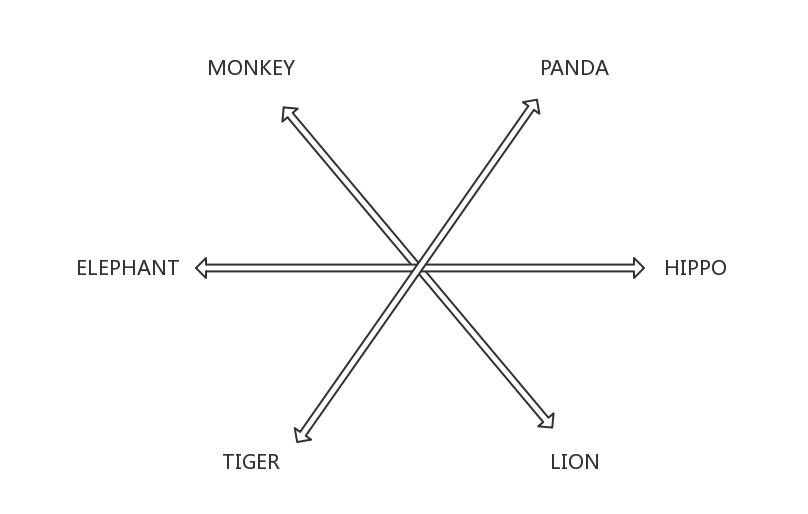
\includegraphics[width=12cm]{fspecies-level-50.png}
					\caption{Free Degree of Species in Senario Level-50} \label{fig:fspecies-level-50}
				\end{figure}
			
				Because each animal's location way is calculated in a similar way, we only use monkeys as an example to illustrate. 
				
				According to those constraints above, we could calculate the $F_{species}$:
				
				
				\begin{equation}
				F(Monkey)=\left\{
				\begin{aligned}
				& F (Monkey, Elephant) & = & 1 \\
				& F (Monkey, Hippoes) & = & 1 \\
				& F (Monkey, Tiger) & = & 1 \\
				& F (Monkey, Pandas) & = & 1 \\
				& F (Monkey, Lion) & = & 0 \\
				& F (Monkey, Monkey) & = & 0
				\end{aligned}
				\right.
				\end{equation}
				
				
				According to those constraints above, we could calculate the $F_{species}$:
				
				\begin{equation}
				F_{spices} = \sum _ { i \in n } \sum _ { j \in m } N (i) \cdot F ( i , j ) = 60
				\end{equation}
				
				Contribution Index can be calculated based on $F_{spices}$ and $F_{choices}$
				
				\begin{equation}
				Contribution\ Index = \frac{F_{choices}}{F_{species}} = \frac{39}{60}
				\end{equation}
				
				
		\subsection{Result of Model}
		
			Because the level setting is a subjective variable, and based on our assumption that there is a simple linear relationship between the level and the difficulty, we use Level-1 and Level-50 to determine the parameters of the equation between level and difficulty.
			
			
			\begin{figure}[h]
				\small
				\centering
				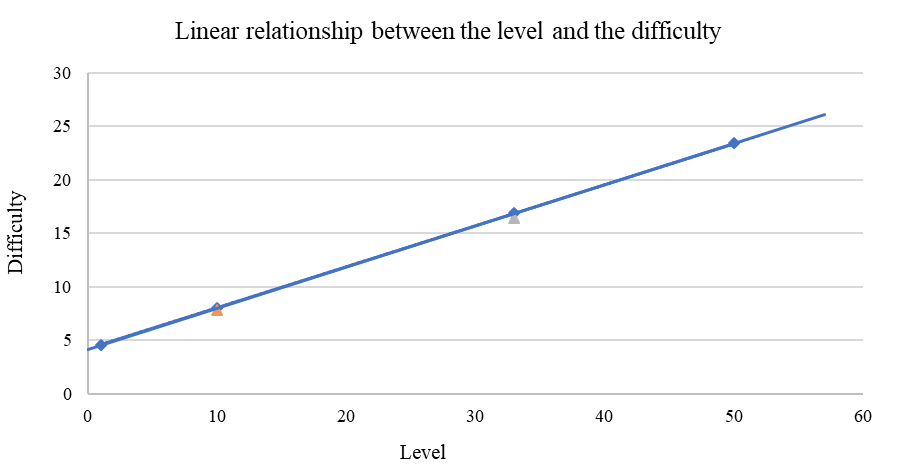
\includegraphics[width=12cm]{linear.png}
				\caption{Linear Equation} 
				\label{fig:linear}
			\end{figure}
		
			The blue line in the figure is the line obtained by using level numbers and difficuly values of the level-1 and level-50. The diamond mark is the normalized result, and the triangle mark is the difficulty value in the real case. We can see through the image that the real value is very close to our standardized results, indicating that we have a linear relationship between the difficulty value and the level. The result of the model is gratifying, indicating that our model is feasible.
			
	
	\section{Improved Search Model based on Free Degree}
	
		In the TASK 2, we want to figure out whether the game has a feasible solution and whether the feasible solution is unique under given constraints.
	
		According to TASK 1, we divide the constraints in the game into two different types: Target-based constraints and Relation-based constraints and use two indicators to represent the effect of different constraints on the difficulty. 
	
		\begin{itemize}
		
			\item Target-based constraints refers to the direct and explicit restrictions of the animal's range of activities (such as Hippo can eat pineapple and orange, Tiger can not eat apples and Strawberries or the Lion must be on the second floor, etc.);
		
			\item Relation-based constraints is the relationship between animals (such as the Tiger on the upper layer of the Cat, the Lion and Monkey are neighbors, etc.).
		\end{itemize}
	
		\clearpage
		
		\begin{figure}[b]
			\small
			\centering
			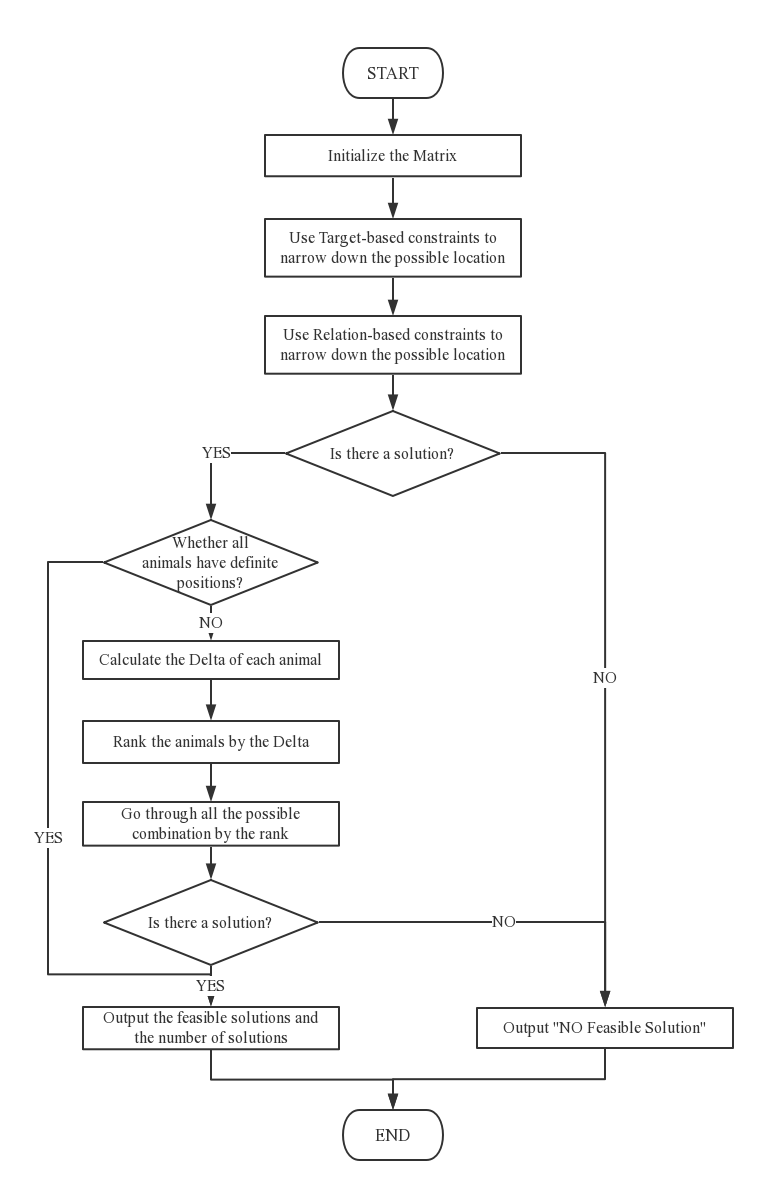
\includegraphics[width=14cm]{process.png}
			\caption{Flowchart of IMSFD} 
			\label{fig:process}
		\end{figure}
	
		\clearpage
	
		
		\subsection{Preliminary}
		
			However, for game "Wonder Island", 9 animals wil be filled in 9 grids. In the unconstrained case, there is a total of $A_9^9=362880$ possibilities. In this case, the general search algorithm finding the feasible solutions is not ideally.
		
			So, we build our algorithm based on dificulty indicators. Let us first explain the impact of these two indicators on the complexity of the algorithm.
			
			\begin{itemize}
				\item Target-based constraints can directly clarify the location of the animal, that is, greatly reduce the complexity of the algorithm.
				
				\item Relation-based constraints while not directly clarifying the location of the animal, but limit the number of feasible solutions. It is equivalent to indirectly reducing the complexity of the algorithm.
				
			\end{itemize}
			
			\textbf{So in this TASK, we optimize the search algorithm based on Free Degree of Choices to better use the information of constraints as much as possible. Based on this, we propose an algorithm: Improved Search Model based on Free Degree.} 
		
		\subsection{ISMFD}
		
			The core idea of the \textbf{I}mproved \textbf{S}earch \textbf{M}odel based on \textbf{F}ree \textbf{D}egree is to first reduce the choice space of each animal by using absolute constraints, and then use the combination of relative constraints and absolute constraints to reduce the possible choice of each animal again. The contribution index is then used to determine the order in which the animal is aligned, thereby maximizing the use of constraints to reduce the time complexity of the algorithm.
			
			
			
			\subsubsection{Use Target-based constraints to narrow down the possible location of each animal}
			
				Initially we assume that for all animals, the possible location, when not considering any constraints, can be represented by the matrix $ [1, 2, 3, 4, 5, 6, 7, 8, 9] $, where 1-9 represent the grid number.
				
				Let's consider a constraint:
				
				\begin{center}
					\emph{"Tiger can't eat apples and strawberries."}
				\end{center}
			
				So, the possible location of tiger narrow down to $ [5, 6, 8, 9] $.
				
				Another instance:
				
				\begin{center}
					\emph{"Tiger is on the second level."}
				\end{center}
				
				So, the possible location of tiger narrow down to $ [2, 3, 4] $.
			
			\subsubsection{Use Relation-based constraints to narrow down the possible location of each animal}
			
				Based on the Relation-based constraints, we can further narrow down the possible location for each animal again.
				
				Let's consider a constraint:
				
				\begin{center}
					\emph{"Lions must go above the cat."}
				\end{center}
				
				So, the possible location of lions narrow down to $ [1, 2, 3, 4] $, because lions cannot be placed at third-level.
				
				Another instance:
				
				\begin{center}
					\emph{"Pandas are the neighbor of Tigers."}
				\end{center}
				
				If the tigers' possible location currently is $ [4] $, and the Pandas' is $ [1, 2, 3] $. According to the constraints, tigers' neighbor is $[1, 3, 9]$, so pandas' possible location narrow down to $[1, 3]$.
				
				The reality is that not all relation-based constraints can reduce the animal's possible location, but some are significant for narrowing it, so we can't ignore the reduction by using relation-based constraints.
			
			\subsubsection{Optimize the search route by using the Free Degree}
			
				After the above two processes, we begin to construct possible alignments. When the number of a species is equal to the number of locations they can be placed, the location of this animal is determined. So we need to first consider such animal species into the permutation.
				
				When, we have considered species which location is determined, can other animal species be considered in an order which can effectively ruduce the time complexity? At this time, if the game not meet the end, then we need to arrange the remaining animals in a certain order and to travel all combinations. 
				
				\textbf{We propose a algorithm based on Free Degree. Free degree of choices can accurately measure the number of combinations. If an animal can reduce the game's Free Degree of Choices(that is, number of combinations is reduced), we should give priority to it. Based on this idea, we constructed the following algorithm:}
				
				\begin{equation}
					Delta_{i} = \frac { \sum _ { i \in n } F_{choices} - F_{choices}^{'} } { n \cdot F_{choices} }
				\end{equation}
				
				Where $i$ is species waited to be located, $n$ is a set of different possible locations for the species, $F_{choices}$ represent Current state of Free Degree of Choices, and  $F_{choices}^{'}$ represent the Free Degree of Choices after locate this species.
				
				Use the instance of Level-33 for detailed explanation:
				
				\begin{figure}[htbp]
					\centering
					\subfigure[Constraints]{
						\begin{minipage}[t]{0.5\linewidth}
							\centering
							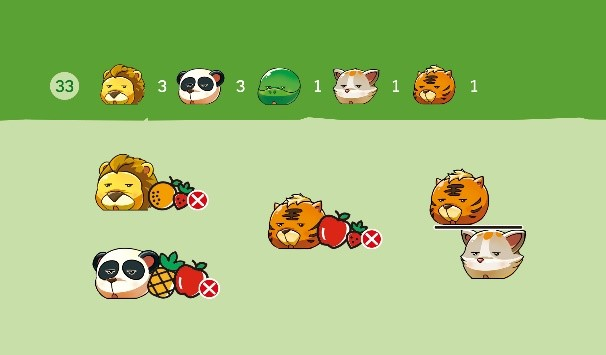
\includegraphics[width=2.5in]{level33.jpg}
							%\caption{fig1}
						\end{minipage}%
					}%
					\subfigure[Game Map]{
						\begin{minipage}[t]{0.5\linewidth}
							\centering
							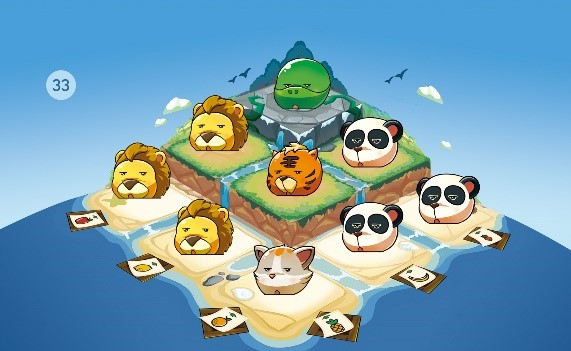
\includegraphics[width=2.5in]{level33-2.jpg}
							%\caption{fig2}
						\end{minipage}%
					}%
					\centering
					\caption{Level-33}
				\end{figure}
			
				The constraints given by the game are:
			
				\begin{itemize}
					\item \emph{"Lions cannot eat neither oranges nor strawberries."}
					\item \emph{"Pandas cannot eat neither pineapples nor apples."}
					\item \emph{"Tigers cannot eat neither apples nor strawberries."}
					\item \emph{"Lions must go above the cat."}
				\end{itemize}
			
				After using two step above to reduce the possible location for each animal, we use the following graph to visualize this process:
				
				\begin{figure}[htbp]
					\centering
					\subfigure[Initial state]{
						\begin{minipage}[t]{0.33\linewidth}
							\centering
							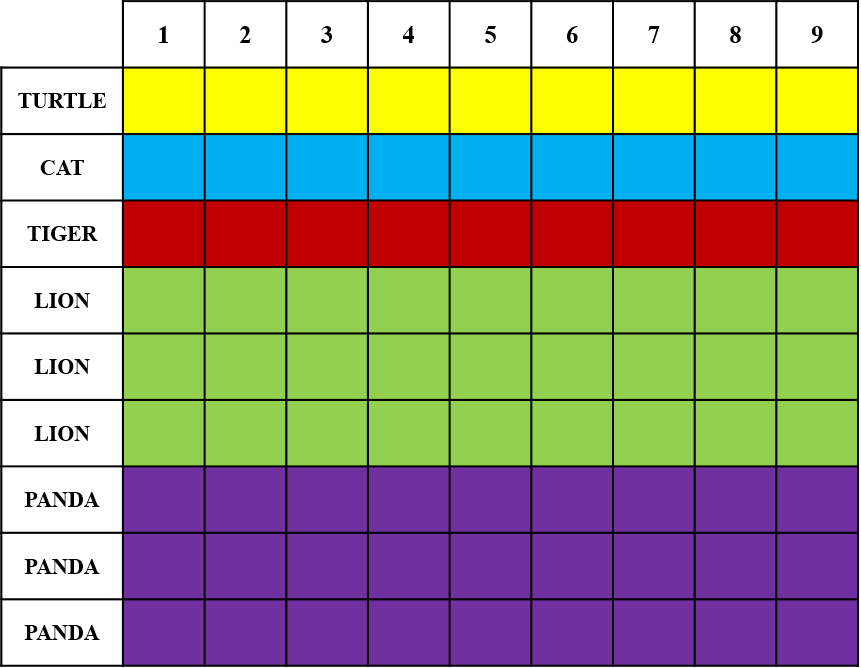
\includegraphics[width=1.5in]{algorithm-1-1.png}
							%\caption{fig1}
						\end{minipage}%
					}%
					\subfigure[Using Target Constraints]{
						\begin{minipage}[t]{0.33\linewidth}
							\centering
							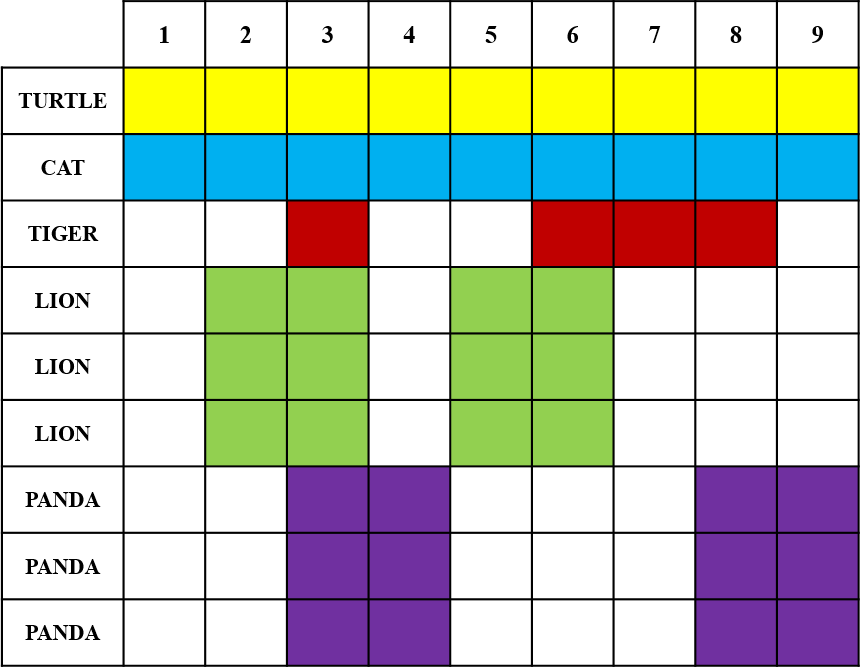
\includegraphics[width=1.5in]{algorithm-1-2.png}
							%\caption{fig2}
						\end{minipage}%
					}%
					\subfigure[Using Relation Constraints]{
						\begin{minipage}[t]{0.33\linewidth}
							\centering
							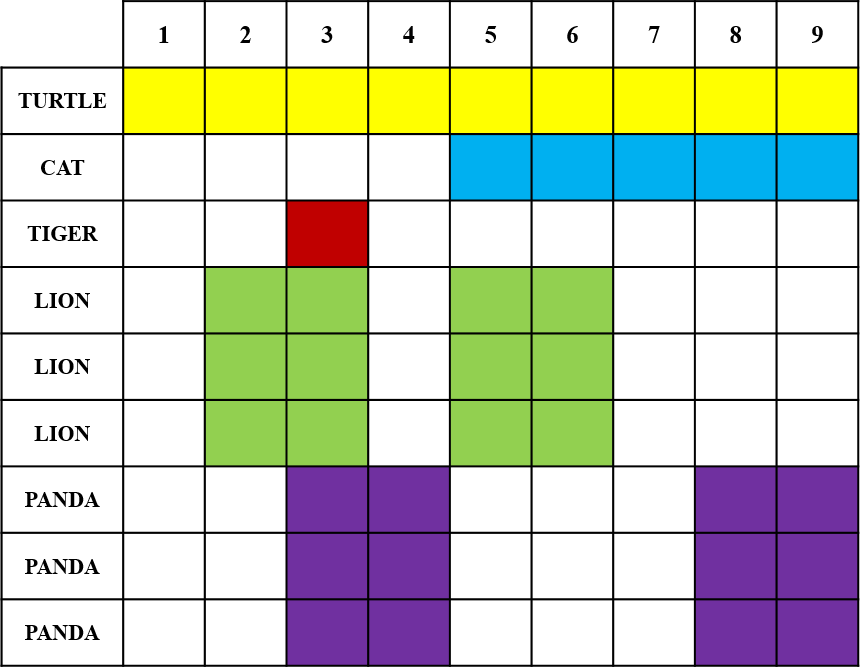
\includegraphics[width=1.5in]{algorithm-1-3.png}
							%\caption{fig2}
						\end{minipage}
					}%
					\centering
					\caption{Changes of Possible Location for Each Animal}
				\end{figure}
			
				From above constraints conbined with the method of narrowing down the possible location for each species, we get following matrix:
				
				\begin{table}[h]
					\centering
					\setlength{\tabcolsep}{3.7mm}
					\begin{tabular}{lccccc}
						\toprule[1.5pt]  %添加表格头部粗线
						Animal Species & Turtle & Cat & Tiger & Lion & Pandas \\
						\midrule  %添加表格中横线
						Species Number & 1 & 1 & 1 & 3 & 3 \\
						Possible Location & $[1, 2,\cdots, 8, 9]$ & $[5,6,7,8,9]$ & $[3]$ & $[2,3,5,6]$ & $[3,4,8,9]$ \\
						\bottomrule[1.5pt] %添加表格底部粗线
					\end{tabular}
				\end{table}
			
				Next we start to calculate the Delta value of each species, and take lions for instance:
				
				\begin{equation}
					F _ { Lion } = S ( \text {Turtle} ) + S ( \mathrm { Cat } ) + S ( \text {Tiger} ) + S ( \text {Panda} ) = 27
				\end{equation}
				
				The possible location for three lions has $C_4^3=4$ possibilities. After we set the position $[2, 3, 5]$ for the lions:
				
				\begin{figure}[htbp]
					\centering
					\subfigure[Before locate lions]{
						\begin{minipage}[t]{0.5\linewidth}
							\centering
							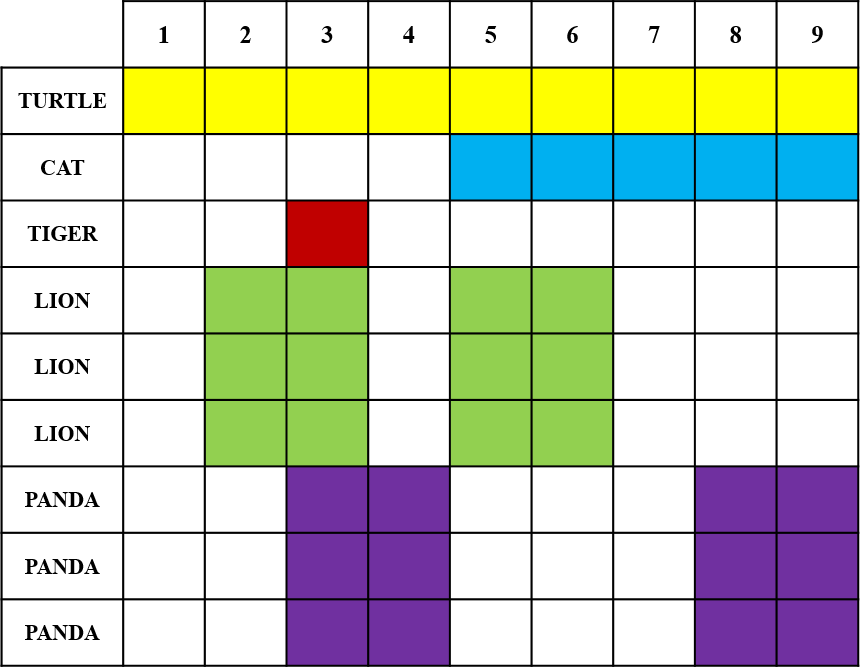
\includegraphics[width=2.5in]{algorithm-1-3.png}
							%\caption{fig1}
						\end{minipage}%
					}%
					\subfigure[Afte locate lions]{
						\begin{minipage}[t]{0.5\linewidth}
							\centering
							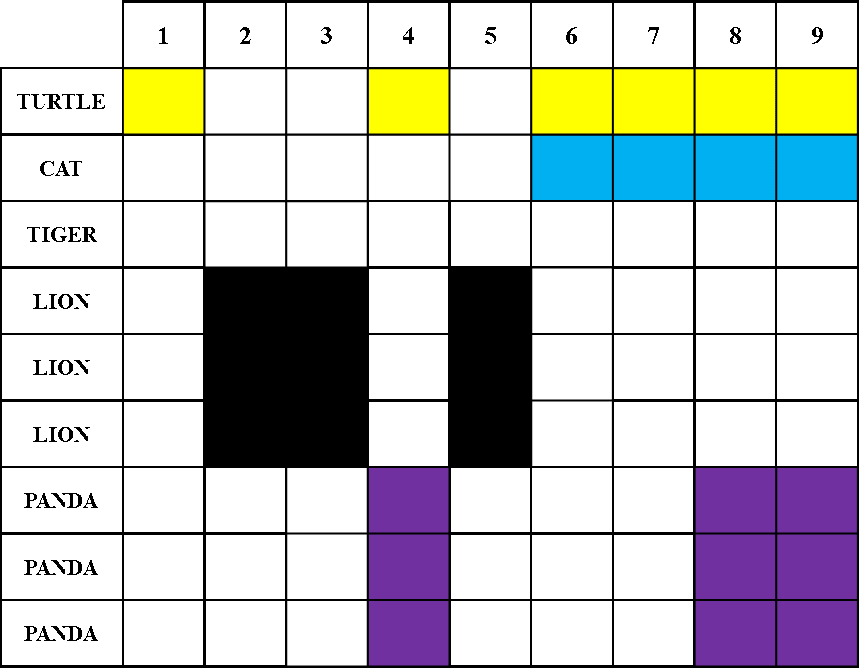
\includegraphics[width=2.5in]{algorithm-1-4.png}
							%\caption{fig2}
						\end{minipage}
					}%
					\centering
					\caption{Changes of Free Degree after locate lions at [2,3,5] }
				\end{figure}
			
				We next calculate the $F _ { Lion }$  after locate lions at $[2,3,5]$.
				
				\begin{equation}
				F _ { Lion[2,3,5] }^{'} = S ( \text {Turtle} ) + S ( \mathrm { Cat } ) + S ( \text {Tiger} ) + S ( \text {Panda} ) = 19
				\end{equation}
				
				We can derive the Free Degree in each case based on the different locations' combinations of the lion:
				
				\begin{table}[h]
					\centering
					\setlength{\tabcolsep}{4mm}
					\begin{tabular}{ccccc}
						\toprule[1.5pt]  %添加表格头部粗线
						Possible Location & $[2,3,5]$ & $[2,5,6]$ & $[2,3,6]$ & $[3,5,6]$ \\
						\midrule  %添加表格中横线
						$F_{choices}^{'}$ & 19 & 22 & 19 & 18 \\
						\bottomrule[1.5pt] %添加表格底部粗线
					\end{tabular}
				\end{table}
			
				Next, Calculate the Delta value of the lion:
			
				\begin{equation}
				Delta_{Lion} = \frac { \sum _ { i \in n } F_{choices} - F_{choices}^{'} } { n \cdot F_{choices} } = 0.25
				\end{equation}
				
				Finally, we can get the Delta of each species( Location of tiger is settled at first two step, so it doesn't have to calculate the Delta):
				
				
				\begin{table}[h]
					\centering
					\setlength{\tabcolsep}{6mm}
					\begin{tabular}{ccccc}
						\toprule[1.5pt]  %添加表格头部粗线
						Species & $Turtle$ & $Cat$ & $Lion$ & $Panda$ \\
						\midrule  %添加表格中横线
						$Delta$ & 0.1111 & 0.1133 & 0.25 & 0.25 \\
						\bottomrule[1pt] %添加表格底部粗线
					\end{tabular}
				\end{table}
			
				So according to the value of Delta from large to small, the combined search order is Tiger-Lion-Panda-Cat-Turtle.
				
				
				
				
				As shown below, according to our planned species selection sequence, the red path is the path we need to traverse, and the black path is the path deleted after the using Relation-based constraints.
				
				\clearpage
				
				\begin{figure}[h]
					\small
					\centering
					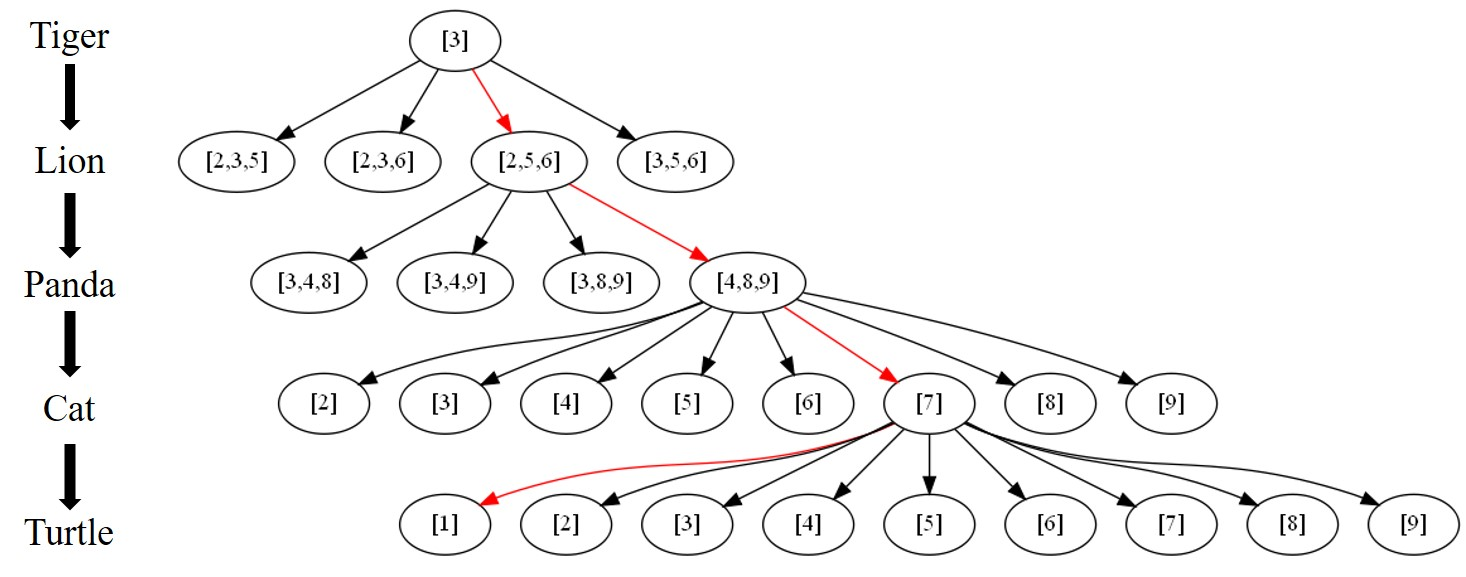
\includegraphics[width=12cm]{path.jpg}
					\caption{Search path using IMSFD} 
					\label{fig:path}
				\end{figure}
			
				To illustrate the effectiveness of our algorithm, we present the search path required if the \textbf{IMSFD} algorithm is not used as a comparison:
				
				Taking the first step of the search path as an example, according to the order of Delta from large to small, our algorithm will consider LION after TIGER. Due to the constraints, the choice of LION is directly limited to [2, 5, 6]; 
				
				However, if there is no improved algorithm  CAT is considered after TIGER, its choices are [2][4][5][6][7][8][9].
				
				\begin{figure}[htbp]
					\centering
					\subfigure[Using IMSFD]{
						\begin{minipage}[t]{0.33\linewidth}
							\centering
							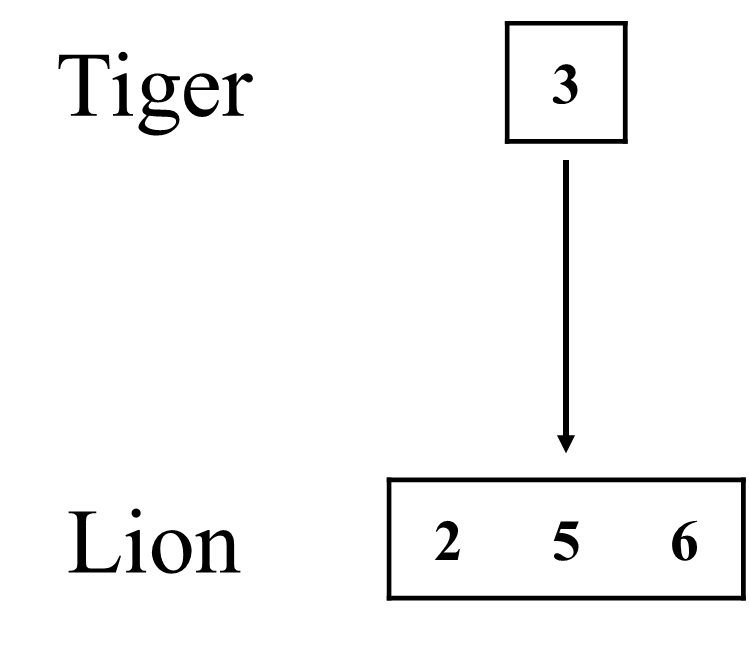
\includegraphics[width=1.38in]{example-1.png}
							%\caption{fig1}
						\end{minipage}%
					}%
					\subfigure[Without IMSFD]{
						\begin{minipage}[t]{0.5\linewidth}
							\centering
							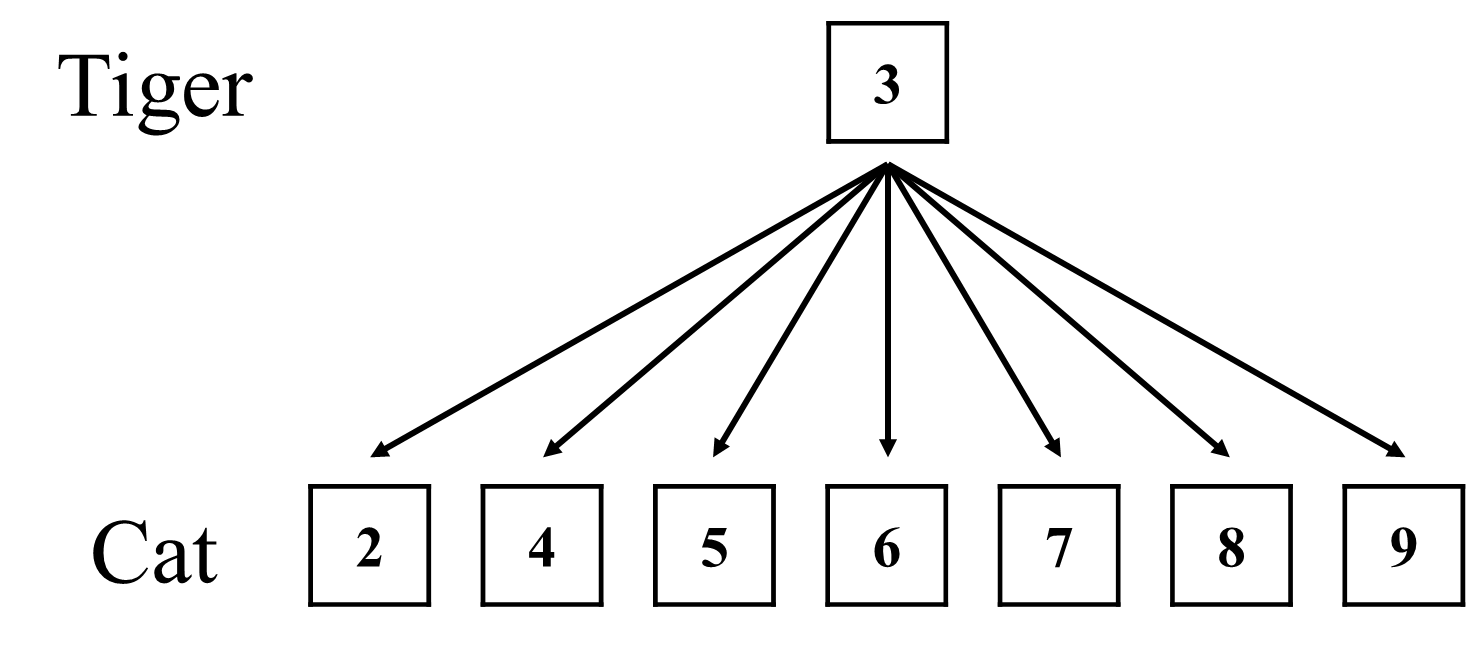
\includegraphics[width=2.6in]{example-2.png}
							%\caption{fig2}
						\end{minipage}
					}%
					\centering
					\caption{Comparison between Using ISMFD or Not}
				\end{figure}
				
				\textbf{ISMFD maximize use of information given by all the constraints based on Free Degree}, which does reduce the combination possibilities and makes the search path more straightforward.
				
				
			
				\begin{figure}[h]
					\small
					\centering
					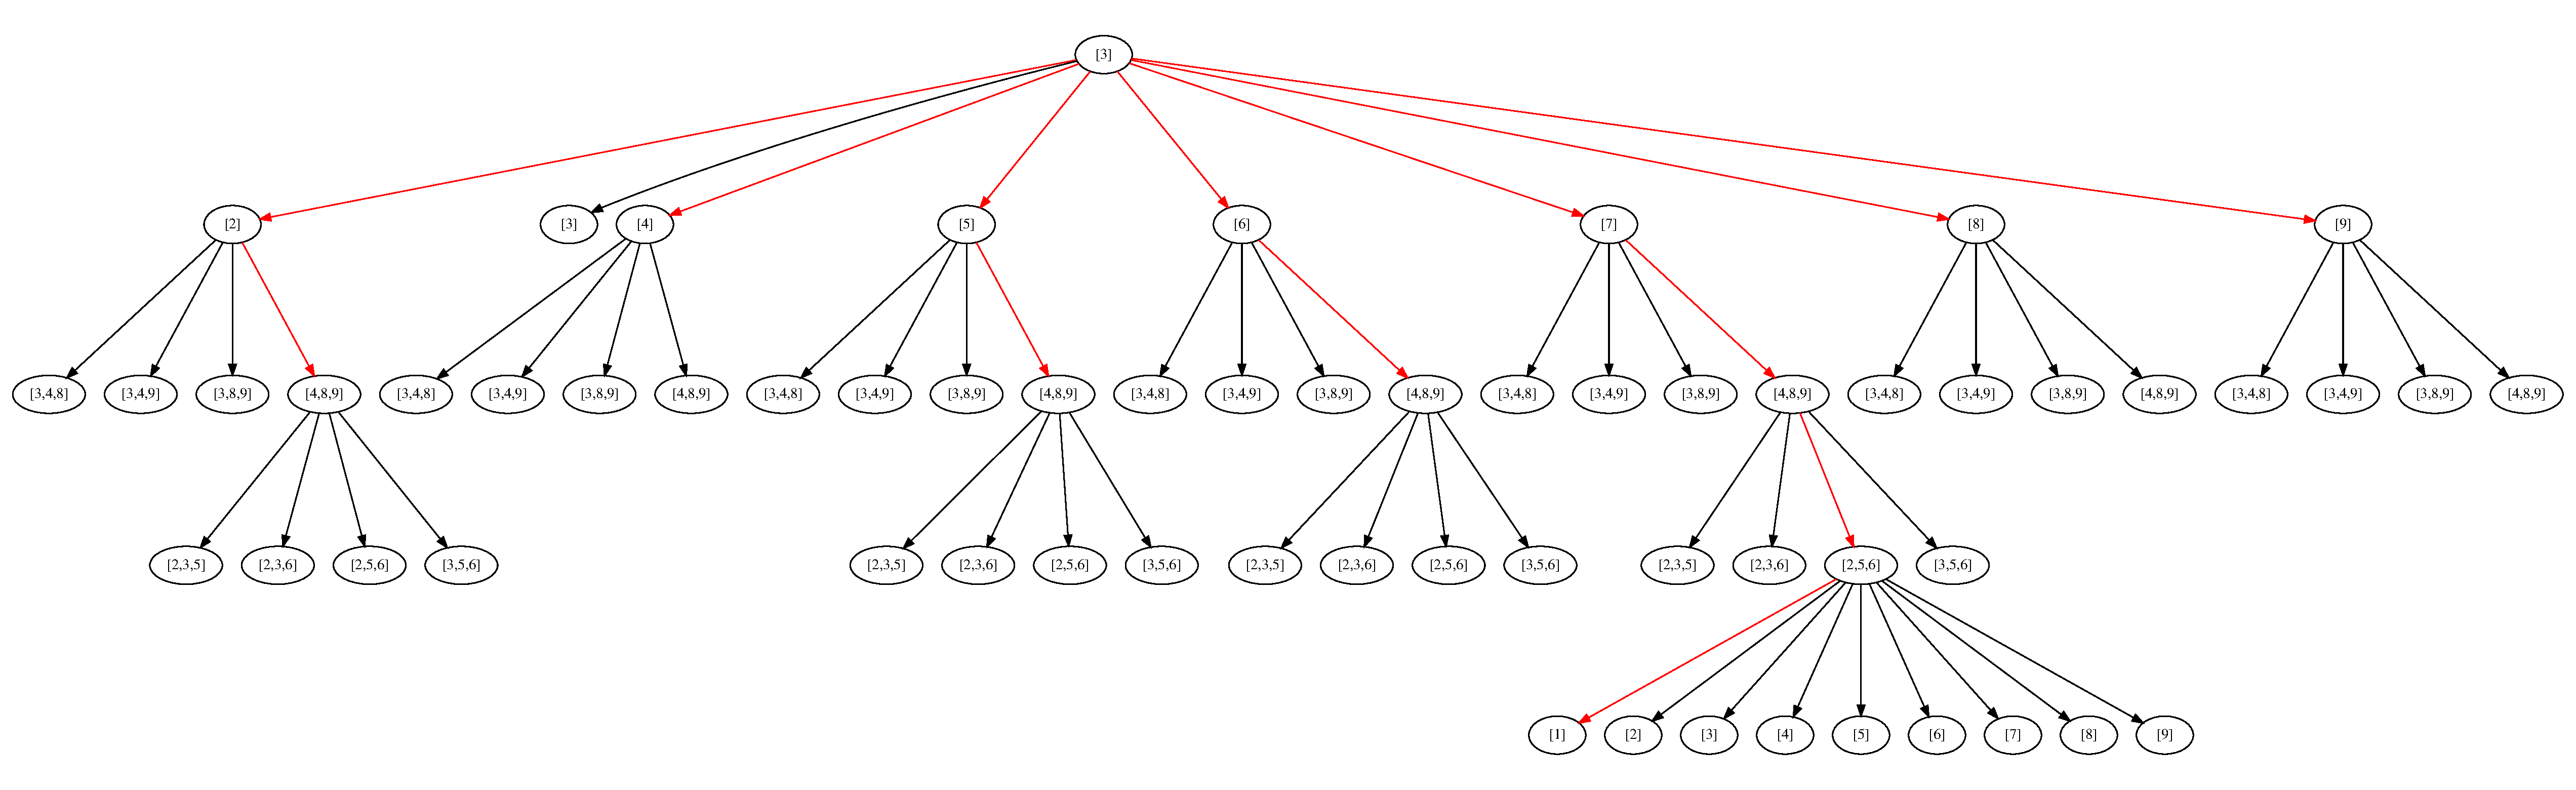
\includegraphics[width=14.5cm]{path-2.eps}
					\caption{Search path without IMSFD} 
					\label{fig:path-2}
				\end{figure}
			
				The complete search path without \textbf{ISMFD} is given above. It is obvious that \textbf{IMSFD} can greatly improve the search efficiency.	
				
				
	\clearpage
	\section{Our New Game: "YES, SIR!"}
	
		\emph{"Welcome, sir! I am the secretary of this city. There will be a city in the future. Now I will help you complete the most basic planning of the city. Because infrastructure is very important for a city, if the infrastructures are well planned, and the entire city will has the opportunity to develop rapidly and sustainably. Improper planning can be devastating for years. I have helped you to divide the city into different areas(blocks), and also found experts in various fields to give you some suggestions on urban construction. I wish that you can build the city better! "}
	
		The game is based on urban planning. When we develop a new city, we need to put infrastructures into various areas of the city, but different infrastructures are not free to be placed in a city. The area will have different attributes and different infrastructures will have different requirements , and there will be corresponding links and logic between the infrastructures. How to properly place these basic infrastructures is a serious issue for social manager.
		
		Specifically, our game has three maps, New York City, Mexico City and Paris City. We divide the city into different blocks(grids) according to the different characteristics of each city.
		
		The player needs to properly and completely plan the infrastructure into the blocks, while at the same time meeting all the planning requirements given by the experts.
		
		\begin{figure}[htbp]
			\centering
			\subfigure[New York City]{
				\begin{minipage}[t]{0.33\linewidth}
					\centering
					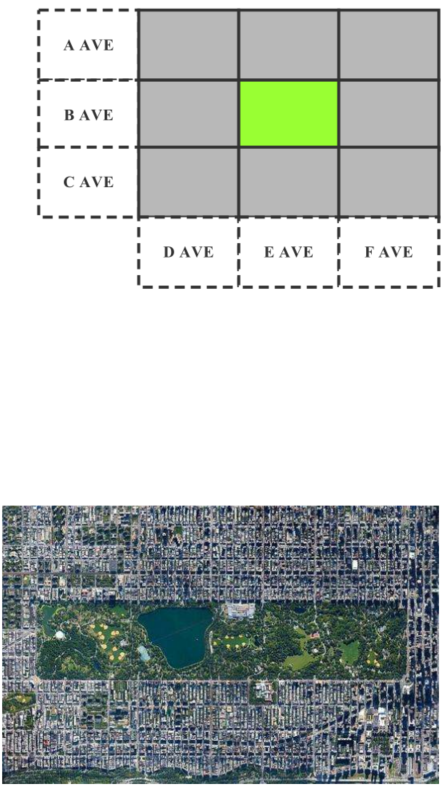
\includegraphics[width=1.5in]{City1.png}
					%\caption{fig1}
				\end{minipage}%
			}%
			\subfigure[Paris]{
				\begin{minipage}[t]{0.33\linewidth}
					\centering
					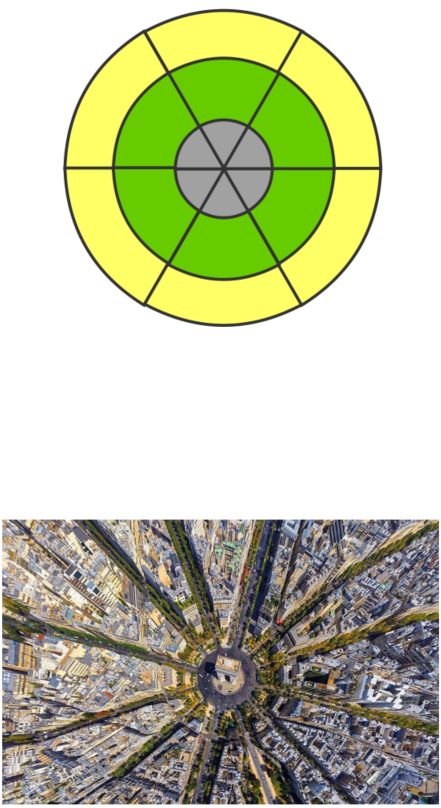
\includegraphics[width=1.5in]{City2.png}
					%\caption{fig2}
				\end{minipage}%
			}%
			\subfigure[Mexico City]{
				\begin{minipage}[t]{0.33\linewidth}
					\centering
					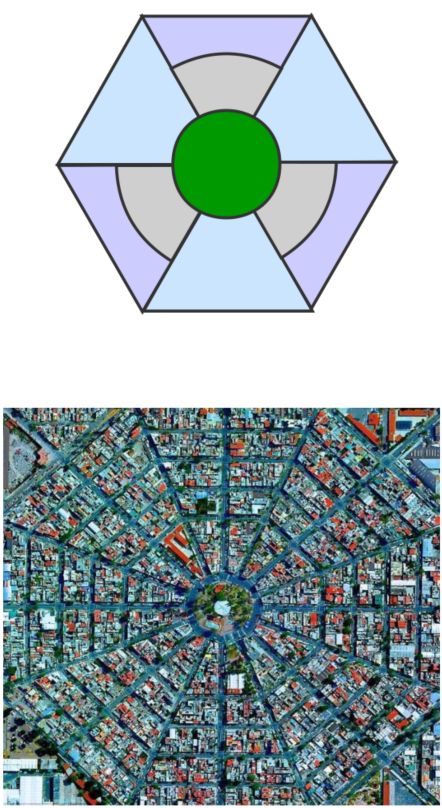
\includegraphics[width=1.5in]{City3.png}
					%\caption{fig2}
				\end{minipage}
			}%
			\centering
			\caption{ Three Maps of "Yes, Sir"}
		\end{figure}
		
		What are the differences between "Yes, Sir" and the "Wonderful Island?"
		
		\begin{itemize}
			\item The background of the game has shifted from the arrangement of animals to city planning.
			
			\item Our background settings are more relevant to life and more realistic, and player can learn more about the infrastructure construction while playing the game.
			
			\item The number of blocks of the map is changable, and the corresponding infrastructure is also changing.
			
			\item There is also a great changing in the shape and association of the blocks, which means that there will be great differences between maps, which will greatly affect the difficulty of the game.
		\end{itemize}
	
		
	
		\subsubsection{Demo}
		
			\begin{figure}[h]
				\small
				\centering
				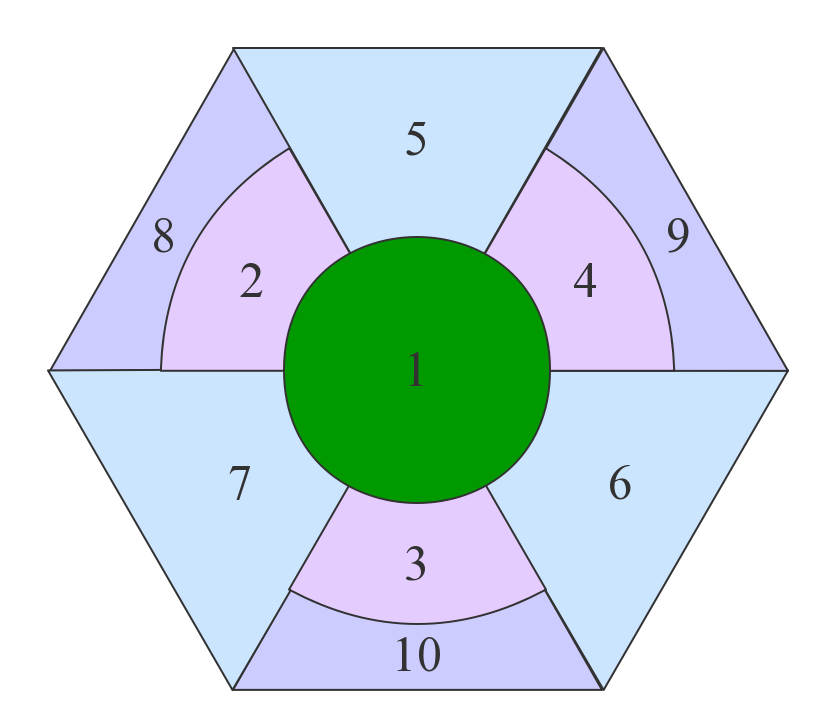
\includegraphics[width=5cm]{demo.png}
				\caption{Map of Maxico} \label{fig:demo}
			\end{figure}
			
			\textbf{We can divide the city into four type of blocks based on geographic location:}
			
			\begin{itemize}
				\item Level One: 1; 
				\item Level Two: 2/3/4
				\item Level Three: 5/6/7
				\item Level Four: 8/9/10
				\item Block 8 is near the highway.
			\end{itemize}
		
			\textbf{And we have to locate ten infrastructures into ten blocks:}
			
			\begin{itemize}
				\item City Government 1
				\item Supermarket 2
				\item School 3
				\item Factory 1
				\item Police Station 1
				\item Fire Station 1
				\item Hospital 1
			\end{itemize}
		
			\textbf{Here is the expert's suggestions:}
		
			\begin{itemize}
				\item Because the city government has to serve the people, it must be arranged at center of the city.
				
				\item The operation of the supermarket should consider saving money as much as possible, so they cannot be arranged at level 1, and because the contents of the two supermarkets have a great relationship with the student supplies, so thay must be arranged at the location of the school adjacent.
				
				\item Because the factory has a large pollution, it can only be arranged in the level 4 area. Considering the cost, the factory should be arranged close to the highway. And in order to take care of the next generation, the factory can't get close to the school.
				
				\item In order to better solve all sorts of problems in various situation and take care of all urban residents, the police station, fire station and hospital must not be in the level 4.
				
			\end{itemize}
			
			
		
	

		

	\section{Sensitivity Analysis}
		
		Because we only have four levels and their constraints, we use cross-validation to verify the robustness of our Difficulty Evaluation Model.
		
		We use any two of the four instances given by paper to determine the relationship between difficulty and level, and then use the other two to evaluate the quality of the model.
		
		\begin{figure}[htbp]
			\centering
			\subfigure[Level 1 \& 10]{
				\begin{minipage}[t]{0.33\linewidth}
					\centering
					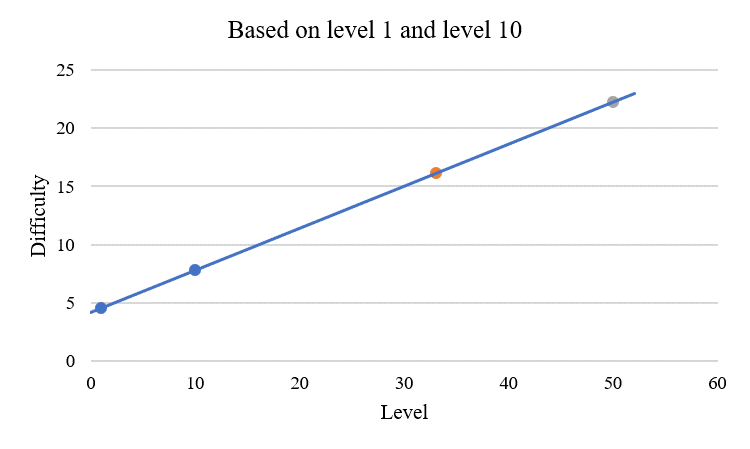
\includegraphics[width=2in]{sensitivity-1.png}
					%\caption{fig1}
				\end{minipage}%
			}%
			\subfigure[Level 1 \& 33]{
				\begin{minipage}[t]{0.3\linewidth}
					\centering
					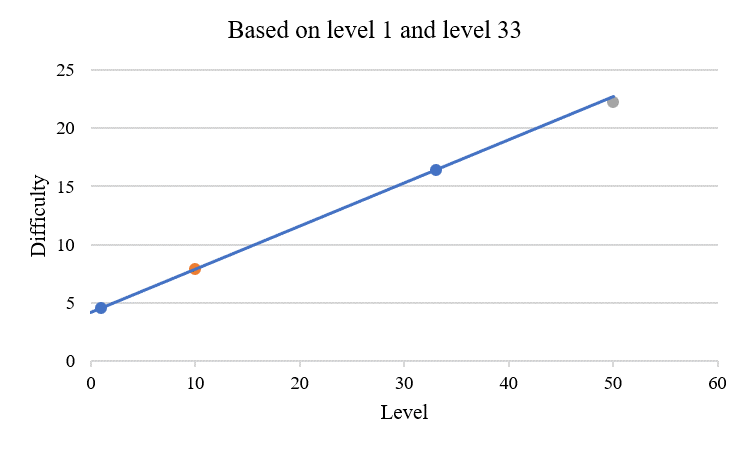
\includegraphics[width=2in]{sensitivity-2.png}
					%\caption{fig2}
				\end{minipage}%
			}%\
			\subfigure[Level 10 \& 33]{
				\begin{minipage}[t]{0.33\linewidth}
					\centering
					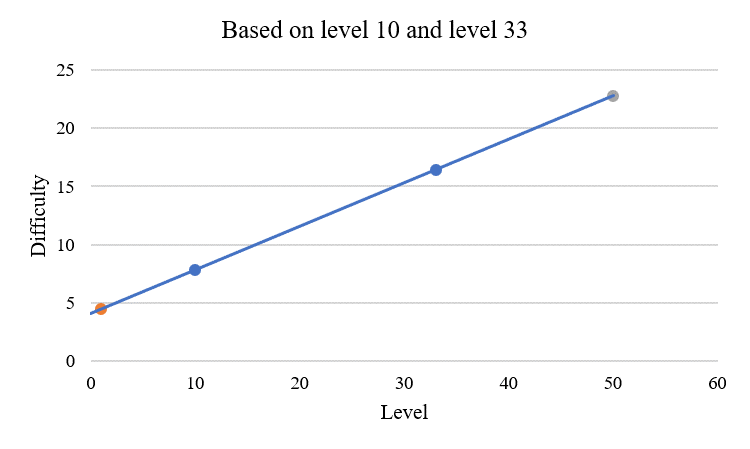
\includegraphics[width=2in]{sensitivity-3.png}
					%\caption{fig2}
				\end{minipage}
			}%
		
			\subfigure[Level 33 \& 50]{
				\begin{minipage}[t]{0.33\linewidth}
					\centering
					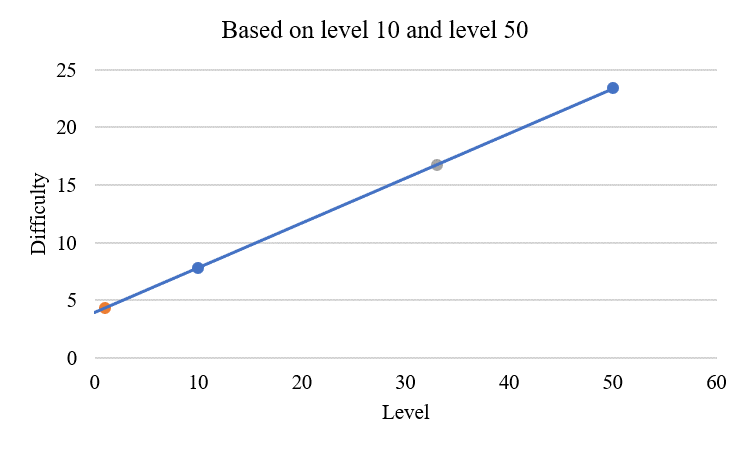
\includegraphics[width=2in]{sensitivity-4.png}
					%\caption{fig2}
				\end{minipage}
			}%
			\quad
			\subfigure[Level 10 \& 50]{
				\begin{minipage}[t]{0.33\linewidth}
					\centering
					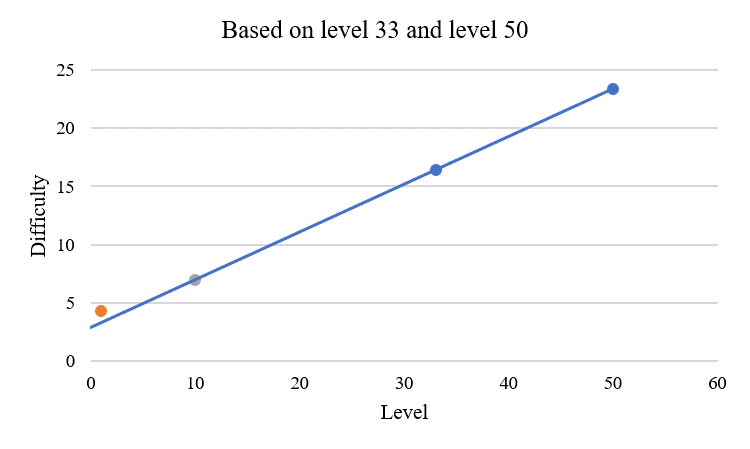
\includegraphics[width=2in]{sensitivity-5.png}
					%\caption{fig2}
				\end{minipage}
			}%
			\centering
			\caption{Sensitivity Anaylsis}
		\end{figure}
	
		The blue dots in the above figures represent the level for training, and the gray and orange dots represent the testing levels.
		
		\clearpage
		
		We can find that the points essentially distribute around the line. We give the deviation between the predicted value and the actual value of the test set in each case as follows:
		
		\begin{table}[htbp]
			\center
			\caption{ Deviation of All Cases}
			
			\setlength{\tabcolsep}{3.6mm}{
			\begin{tabular}{lcccccc}
				\toprule[1.5pt]  %添加表格头部粗线
				Training Level & 1\&10 & 1\&33 & 1\&50 & 10\&33 & 10\&50 & 33\&50\\
				\midrule  %添加表格中横线
				Deviation-1 & 1.763\% & 1.040\% & 2.631\% & 3.473\% & 4.509\% & 27.872\% \\
				Deviation-2 & 4.796\% & 2.900\% & 2.698\% & 2.643\% & 2.164\% & 10.681\% \\
				\bottomrule[1.5pt] %添加表格底部粗线
			\end{tabular}}
		\end{table}
	
		From our calculation results, we can see that the deviation values calculated by our model are mostly within 10\%, and majority are less than 3\%. Explain that our model is robust and can define difficulty in small data volume(We just need two instance to normalize the relation between difficulty and the level).
		
		At the same time, the table also reflects some problems with our model. When we know the difficulty of the high-level, the model may not be able to calculate the difficulty of low-level accurately.
		
		
		
		
		
		
		
		
	\section{Strengths and Weaknesses}
	
		\subsection{Strengths}
		
			\begin{itemize}
				
				\item Our Difficulty Evaluation Model can judge the difficulty without simulating the process of solving the problem. \\
				\item Our difficulty Evaluation Model can measure the difficulty from an objective perspective, eliminating the subjective influence of people. \\
				\item Our model represent the practical meaning of constraints into a contribution index that can be described in mathematical language. \\
				\item ISMDF uses the Free degree of Choices to maximize the use of the constraints, greatly reducing the time required to solve problem. \\
		
			\end{itemize}
		
		\subsection{Weaknesses}
		
			\begin{itemize}
				
				\item The data used to determine the difficulty indicators and level is too small to fully explain that the relationship between the two must be linear. \\
				\item In some extreme circumstances, it may happen that the Delta cannot shorten the solution time. \\
				
			\end{itemize}
		
	\nocite{*}
	\bibliography{cnki}
		
	\clearpage
	\section{Memo of Promotion for Our Game}
	
		\begin{center}
			\Large\textbf{NEW GAMES: YES, SIR!}
			
			\emph{To all interested users}
		\end{center}
		
		\textbf{Game Introduction}
		
		"Yes sir!" is a game that exercise your logic analysis ability. It is based on city planning and transforms the areas of a city into blocks. Then you need to properly locate different infrastructures in the city as experts' required.
		
		\textbf{Why choose "Yes, Sir!"?}
		
		The game can cultivate children's diversified thinking modes; it can also help adults to relieve stress and strengthen analytical skills; For the elderly, the biggest effect of this game is to train the brain to avoid some elderly diseases, thus effectively extending the life. 
		
		\textbf{What are the advantages of the game?}
		
		The game has a diversified board. Each board is designed according to the real city planning. At the same time, the constraints in our game are based on real-life constraints. So while playing our game, you will also experience the hardships and difficulties of being a city planner. Of course, you can also feel the feeling of controlling everything.
		
		In the basic phase of the game, you will be assigned some very simple urban models, and you can achieve a reasonable allocation of the infrastructure with a simple match. As the game progresses, the cities you face become more and more complex, and you need to consider more and more situations. We have a rich board system, from the rules of the board to the irregular shape of the board, and this At the same time, the number and variety of infrastructures you need to secure are constantly increasing, and the need for your logical thinking skills is greater.
		
		Someone may ask, is it difficult to set the difficulty of your question? Will there be a situation in which the difficulty suddenly rises? We have a professional difficulty assessment system, and the assessment of the difficulty of the topic is based on the existing mathematical model. Each topic will have a corresponding difficulty factor. The difficulty level of each topic is very detailed and more reasonable.
		
		\textbf{"YES, SIR" is suitable for all ages. Without spending the lots of money, but can enhance the parent-child relationships, won't it?}

\end{document}
